\chapter{Odpowiedź skokowa na potrzeby DMC}
W tym rozdziale opisany został eksperyment zbierania odpowiedzi skokowej,
przystosowanej do wykorzystania przy projektowaniu regulatora DMC dla obiektu.
Polegał on na przeprowadzeniu skoku z punktu pracy obiektu, czyli przy
wartości sterowania $U = 0,9$, do górnego ograniczenia sygnału sterującego,
czyli $U = 1,2$. Następnie odpowiedź została znormalizowana, czyli przesunięta
o wartość wyjścia w punkcie pracy, oraz podzielona o długość
skoku sterowania.
\begin{equation}
  Y(k) = (Y_{eksperymentu}(k) - Y_{pp})/\Delta U
\end{equation}
Wyniki zostały przedstawione na wykresie \ref{fig:skok_DMC}. Widać na nich
poprawność wyliczonego w rozdziale \ref{sec:zad2} wzmocnienia statycznego.
\begin{figure}
  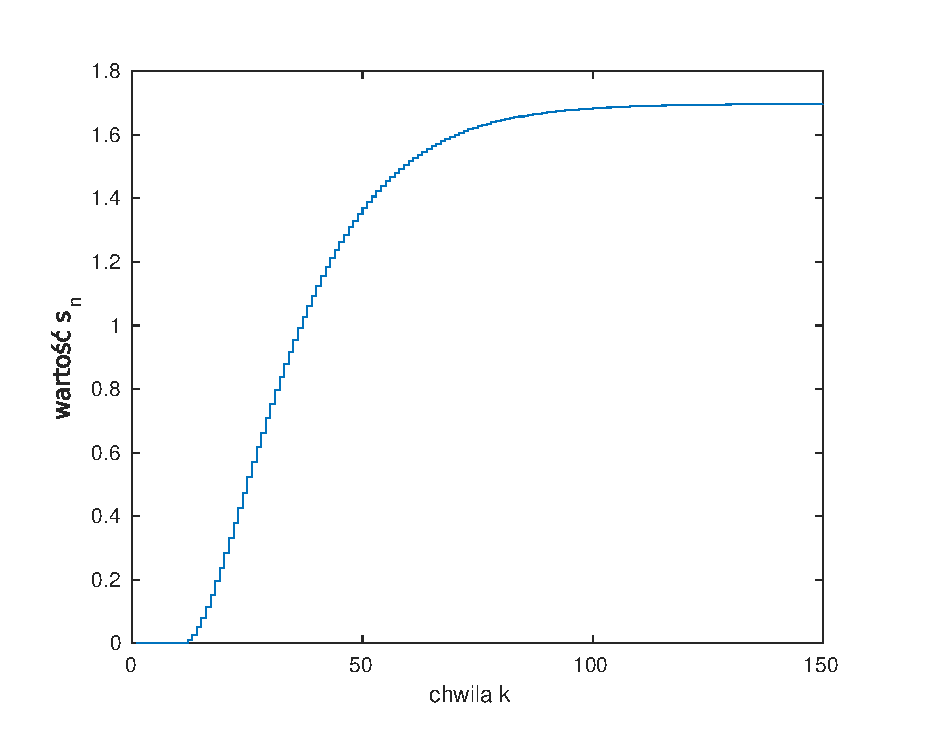
\includegraphics{wykresy/3.eps}
  \caption{Odpowiedź skokowa znormalizowana na potrzeby algorytmu DMC}
  \label{fig:skok_DMC}
\end{figure}
